% figure: 现控1-5-模拟结构图.png
% Two integrators, two feedback terms, and the direct feedthrough term.
\documentclass[border=10pt]{standalone}
\usepackage{fontspec}
\setmainfont{Cambria}
\usepackage{unicode-math}
\setmathfont{Cambria Math}
\usepackage{tikz}
\usetikzlibrary{arrows.meta}
\begin{document}
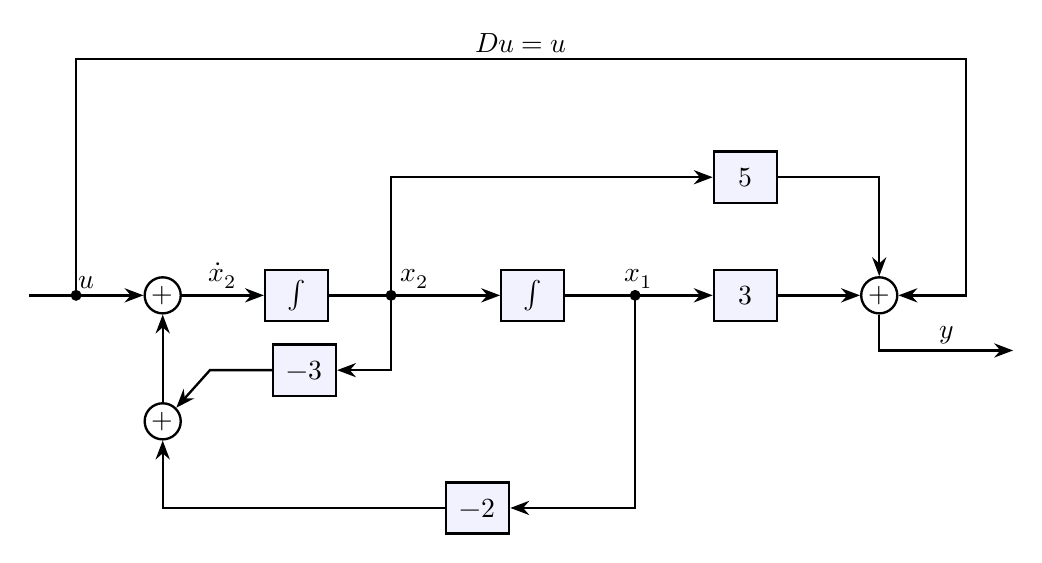
\begin{tikzpicture}[>=Stealth,line width=0.85pt,
 b/.style={draw,minimum width=0.8cm,minimum height=0.65cm,fill=blue!5},
 sum/.style={draw,circle,inner sep=1pt,minimum size=0.4cm},
 lab/.style={fill=white,inner sep=2pt},dot/.style={circle,fill,inner sep=1.4pt}]
\node[sum] (s) at (0,0) {$+$};
\node[b] (i2) at (1.7,0) {$\int$};
\node[b] (i1) at (4.7,0) {$\int$};
\node[b] (g3) at (7.4,0) {$3$};
\node[sum] (o) at (9.1,0) {$+$};
\node[sum] (f) at (0,-1.6) {$+$};
\node[b] (m3) at (1.8,-0.95) {$-3$};
\node[b] (m2) at (4,-2.7) {$-2$};
\node[b] (g5) at (7.4,1.5) {$5$};
\draw[->] (-1.7,0) -- node[lab,above] {$u$} (s);
\draw[->] (s) -- node[lab,above] {$\dot x_2$} (i2);
\draw[->] (i2) -- node[lab,above] {$x_2$} (i1);
\draw[->] (i1) -- node[lab,above] {$x_1$} (g3);
\draw[->] (g3) -- (o);
\draw[->] (o.south) -- (9.1,-0.7) -- node[lab,above] {$y$} (10.8,-0.7);
\node[dot] at (2.9,0) {};
\node[dot] at (6,0) {};
\node[dot] at (-1.1,0) {};
\draw[->] (2.9,0) -- (2.9,-0.95) -- (m3.east);
\draw[->] (m3.west) -- (0.6,-0.95) -- (f.north east);
\draw[->] (6,0) -- (6,-2.7) -- (m2.east);
\draw[->] (m2.west) -- (0,-2.7) -- (f.south);
\draw[->] (f.north) -- (s.south);
\draw[->] (2.9,0) -- (2.9,1.5) -- (g5.west);
\draw[->] (g5.east) -- (9.1,1.5) -- (o.north);
\draw[->] (-1.1,0) -- (-1.1,3) -- node[lab,above] {$Du=u$} (10.2,3) -- (10.2,0) -- (o.east);
\end{tikzpicture}
\end{document}
